\section{Vererbung (Inheritance)}
	Vererbung ist ein Konzept, das es erlaubt, neue Klassen auf Basis von alten Klassen zu definieren. Die neuen (Unter-, Sub-) Klassen besitzen, ohne Eingriffe in den
	Sourcecode der bereits bestehenden (Ober-, Basis-, Super-) Klassen, all deren Eigenschaften, sie $erben$ deren Verhalten und Daten. Den Vorgang der Vererbung nennt man $Ableiten$.\linebreak
	\begin{minipage}[t]{7 cm}
		\subsection{Einsatz der Vererbung \verweiscpp{13.1}}
		\begin{compactitem}
			\item Bestehende Klassen erweitern (zus�tzliche Attribute und Elementfunktionen)
			\item Bestehende Methoden einer Basisklasse �ndern (�berschreiben)
			\item Einsatz nur wenn eine \textbf{IST-EIN (is a)} Beziehung besteht (z.B. Baum \textbf{ist eine} Pflanze, Blume \textbf{ist eine} Pflanze)
			\linebreak
		\end{compactitem}
		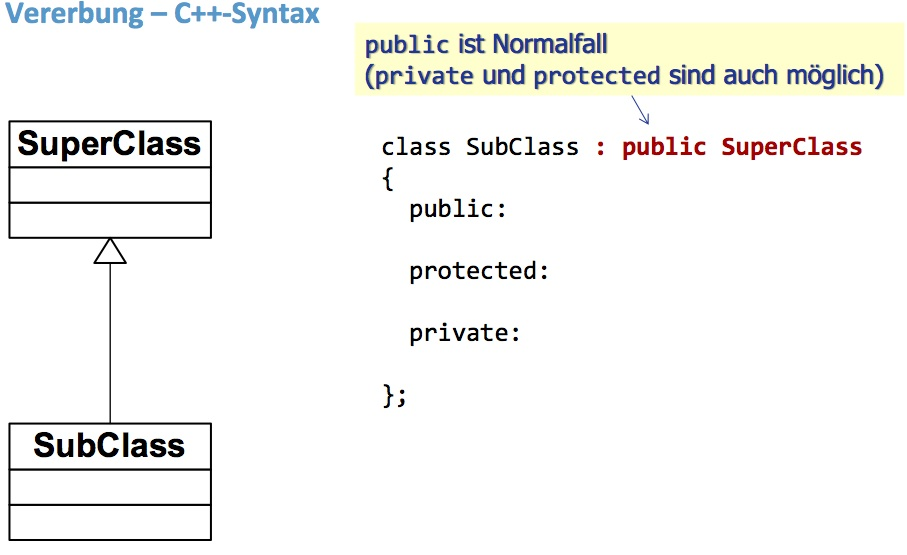
\includegraphics[width=1\textwidth]{pics/bsp_Vererbung.jpg}
		\subsection{Ableiten einer Klasse \verweiscpp{13.2}}
			Der Syntax der Ableitung einer Klasse ist oben aufgef�hrt. Als weiteres Beispiel ist im Anhang das Beispiel des ComicCharacters und SuperHero eingef�gt. SuperHero \textbf{ist ein} ComicCharacter.
			\begin{compactitem}
				\item friend-Beziehungen werden nicht vererbt
				\item Ein Objekt einer Oberklasse kann Objekte einer beliebigen Unterklasse aufnehmen
				\item Ein Objekt einer Unterklasse kann keine Objekte der Oberklasse aufnehmen
				\item Ein Objekt einer vererbten Klasse enth�lt alle Teile der Basisklasse und zus�tzlich noch die spezifischen eigenen Teile.
				\item Das Objekt ist somit mindestens so gross wie jenes der Basisklasse (es gibt keine Vererbung $by$ $reference$)
				\linebreak
			\end{compactitem}
			\lstinputlisting[language=C++,tabsize=2]{code/substitutionsprinzip.cpp}
	\end{minipage}	
	\hspace*{0.5cm}
	\begin{minipage}[t]{11.5 cm}
	\subsection{Zugriff auf Elemente der Basisklasse \verweiscpp{13.6}}
		\textbf{Bei Vererbung mit public (Normalfall):}
			\begin{compactitem}
				\item Zugriff m�glich auf alle public- und protected- Elemente der Basisklasse, die Zugriffsrechte 
				(public, protected) der Basisklasse werden in der abgeleiteten Klasse beibehalten
				\linebreak
			\end{compactitem}
		\textbf{Bei Vererbung mit protected:}
			\begin{compactitem}
				\item Zugriff m�glich auf alle public- und protected- Elemente der Basisklasse, die Zugriffsrechte 
				von public und protected der Basisklasse werden in der abgeleiteten Klasse zu protected
				\linebreak
			\end{compactitem}
		\textbf{Bei Vererbung mit private:}
			\begin{compactitem}
				\item Zugriff m�glich auf alle public- und protected- Elemente der Basisklasse, die Zugriffsrechte 
				von public und protected der Basisklasse werden in der abgeleiteten Klasse zu private
				\linebreak
			\end{compactitem}
		\textbf{Bei allen drei: kein Zugriff auf private-Elemente der Basisklasse}
		\lstinputlisting[language=C++,tabsize=2]{code/privateFehler.cpp}
	\subsection{Slicing Problem \verweiscpp{13.3}}
		Links: Beim Kopieren werden nur die ComicCharacter-Teile ber�cksichtigt. Durch das Kopieren wird alles �berfl�ssige weggeschnitten, �brig bleibt ein reines ComicCharacter Objekt im Fall von s f�hrt dies dazu, dass die erweiterten SuperHero Daten und Funktionen verloren gehen.\newline
		Rechts: Hier wird dank des Referenzparameters der gesamte Superheld ausgegeben.\newline
		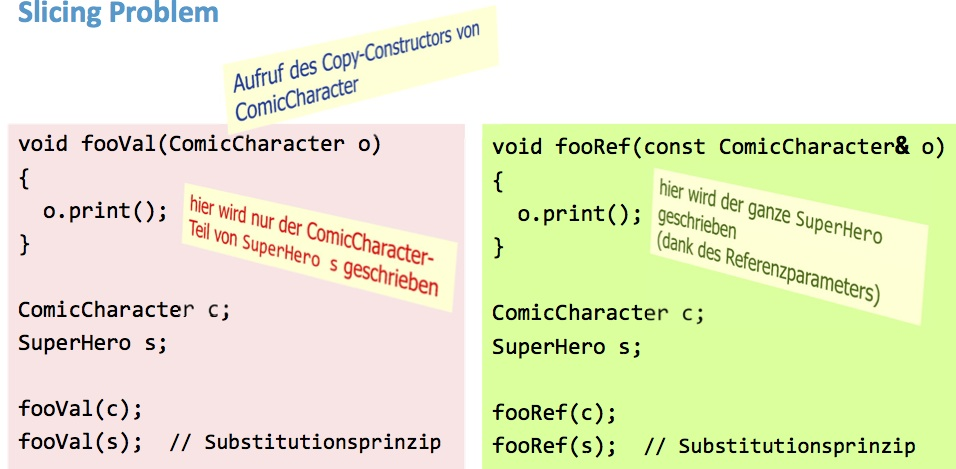
\includegraphics[width=1\textwidth]{pics/SlicingProblem.jpg}
	\end{minipage}	
\newpage
	\subsection{Vererbung und G�ltigkeitsbereiche \verweiscpp{13.4}}
		Die Klasse C enth�lt alle Elemente von B und somit auch von A. A jedoch hat kein i un kann auch von keiner Oberklasse erben, dies ergibt den Fehler. B hat zwar auch kein j, erbt aber das von A.\newline
		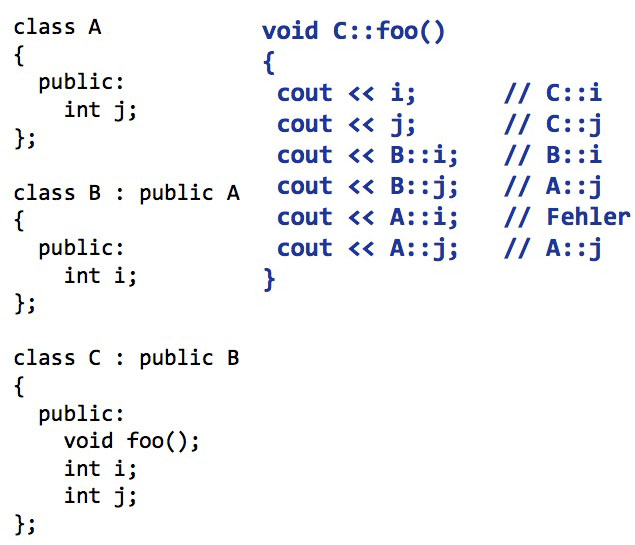
\includegraphics[width=0.6\textwidth]{pics/zugriffVererbung.jpg}
	\subsection{Elementfunktionen bei abgeleiteten Klassen \verweiscpp{13.5}}
	\begin{minipage}[t]{12 cm}
    	\subsubsection{Konstruktoren\verweiscpp{13.5.1}}
    		In einem Konstruktor m�ssen alle Elemente eines Objekts (auch die ererbten) initialisiert werden. Folgendes Beispiel zeigt die direkte Initialisierung aller Elemente. Vor allem bei grossen oder mehreren Klassen ist dies nicht zielf�hrend. Stattdessen wird das Chaining Prinzip angewandt. Falls kein Aufruf eines Basislklassen-Konstruktors in der Initialisierungsliste eines Konstruktors erscheint, so f�gt der Compiler automatisch den Default-Konstruktor der Basisklasse ein.
   			\lstinputlisting[language=C++,tabsize=2]{code/initVererbungKonstruktor.cpp}
   		\subsubsection{Chaining}
   			Jede Klasse erledigt nur die eigenen Aufgaben. Aufgaben, die ererbte Methoden �bernehmen k�nnen, werden diesen delegiert (Aufruf der jeweiligen Konstruktoren)\newline
   			\textbf{Wichtig: die Elemente der Basisklasse m�ssen immer als erste initialisiert werden}
    		\lstinputlisting[language=C++,tabsize=2]{code/initVererbungChaining.cpp}
	\end{minipage} \hspace*{0.5cm}
	\begin{minipage}[t]{6.5 cm}
		\subsubsection{Copy-Konstruktor \verweiscpp{13.5.2}}
			\begin{compactitem}
				\item Wenn kein Copy Constructor explizit definiert wird, so erzeugt das System einen
				\item Darin wird immer (ebenfalls automatisch) zuerst der Copy Constructor der Basisklasse aufgerufen
				\linebreak
			\end{compactitem}
		\subsubsection{Destruktor \verweiscpp{13.5.3}}
			\begin{compactitem}
				\item Auch Destruktoren werden nach dem Chaining-Prinzip aufgebaut
				\item Jede Klasse k�mmert sich um die eigenen Attribute und �berl�sst jene der
				Basisklasse auch der Basisklasse
				\item Destruktoren m�ssen nie explizit aufgerufen werden. Der Destruktor der
				Basisklasse wird \textbf{am Schluss} des Destruktors immer automatisch aufgerufen\newline
				Ein leerer Destruktor der Art
				\lstinputlisting[language=C++,tabsize=2]{code/destructor.cpp}
				ruft automatisch den Basisklassen-Destrukor (von ComicCharacter) auf.
				\linebreak
			\end{compactitem}
		\subsubsection{�berschreiben von ererbten Methoden\verweiscpp{13.5.3}}
			\begin{compactitem}
				\item Falls ererbte Methoden nicht das erf�llen, was eine bestimmte Klasse m�chte, dann
				k�nnen diese Methoden neu definiert (�berschrieben) werden.
				\item Methoden, welche in einer abgeleiteten Klasse �berschrieben werden k�nnen, m�ssen in der Basisklasse mit virtual gekennzeichnet sein.
				\item Im Anhang wird dieses �berschreiben einer Methode beim SuperHero f�r die Funktion $dance()$ vorgenommen. W�hrend ein normaler ComicCharacter tanzt, wird diese Funktion beim SuperHero �berschrieben und mit tanzt nicht �berschrieben.
				\linebreak
			\end{compactitem}

		
	\end{minipage}

    
	